\documentclass[a4paper, titlepage]{article}
\usepackage[T1]{fontenc}
\usepackage[swedish]{babel}
\usepackage[utf8]{inputenc}
\usepackage{graphicx}
\usepackage[normalem]{ulem}
\title{
    Programming Project \\
    C++ Programming(EDA031)
}
\author{
        Department of Computer Science \\
            \\
        Simon Thörnqvist (ada09st1@student.lu.se)
            \and
        Fredrik Pettersson (ada09fpe@student.lu.se)
            \and
        Marcus LindFeldt (ada08mli@student.lu.se)
            \and
        [Robobuilder enter name and email here]
}
\date{\today}
\begin{document}
\maketitle

\section{Introduction}\label{introduction}
The purpose of this project was to implement a news system similar to the Usenet News. The assignment included the implementation of the server, the client and the communication between them. NNTP was the protocol used for the communication.

\section{Requirements}\label{requirements}
We believe that all requirements have been fulfilled.

\section{System Outline}\label{systemoutline}
\subsection{Com}

\subsection{Database}
\subsubsection{In Memory}
This implementation of the database stores the information in the primary memory and destroys it when the server is terminated. It simply uses a map to store the newsgroups where the key is the id number of the newsgroup. Each newsgroup has it's own map to store their articles and the key is the id number of the article. Articles store the title, author and text as strings.

\subsubsection{File}

\subsection{Server}

\subsection{Client}

\section{Communication}

\section{Summary}\label{summary}

\newpage
\appendix
\section{UML Diagram}\label{App:AppendixA}
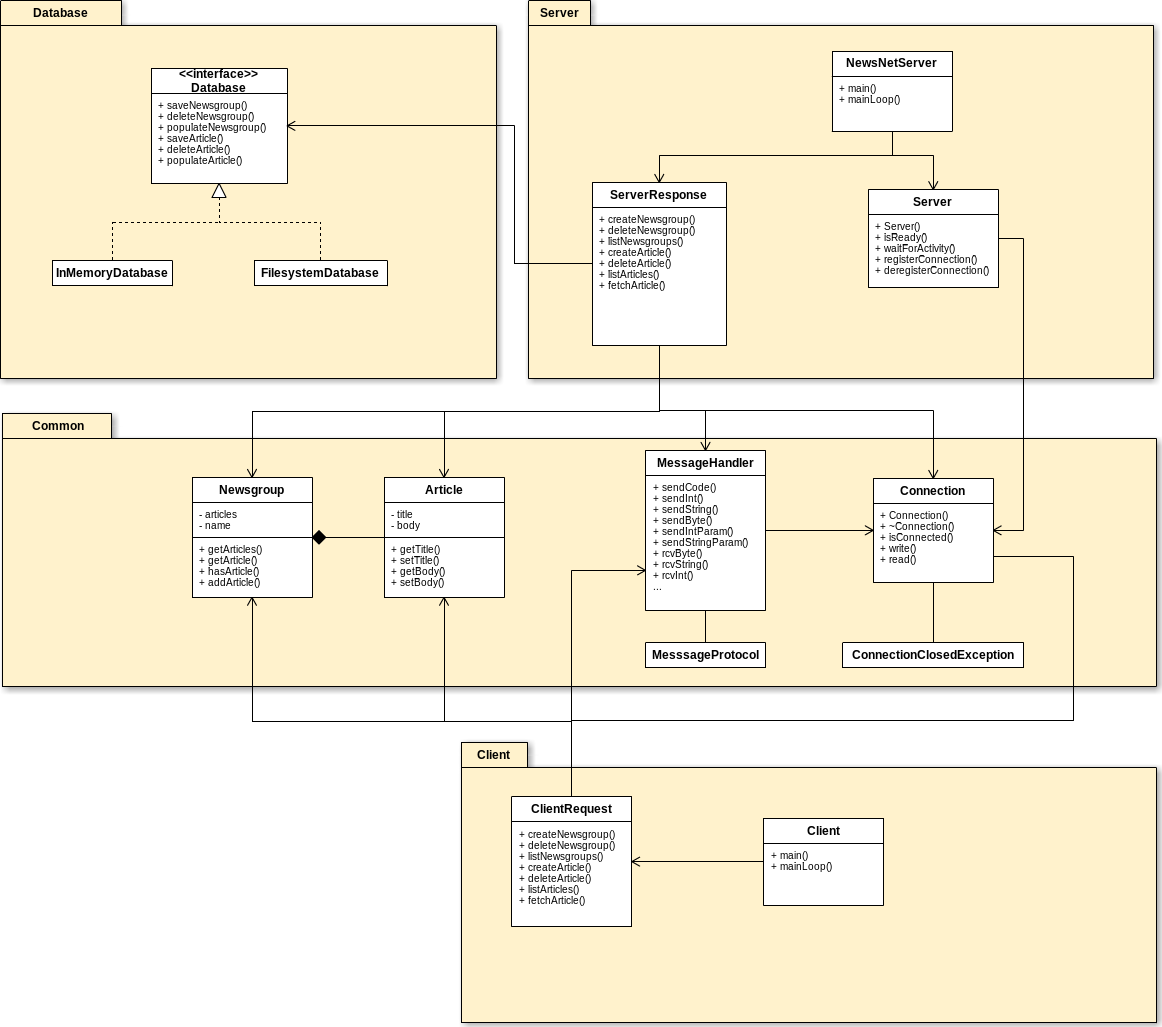
\includegraphics[width=130mm]{NewsNet_UML.png}

\end{document}